\section*{\centering ДҮРС ТАНИХ ТЕХНОЛОГИД СУУРИЛСАН МОНГОЛ БИЧГИЙН СУРГАЛТЫН АППЛИКЕЙШН}
\addcontentsline{toc}{section}{Товчлол}

\begin{flushright}
\deptname\\
Оюутан: \authorcode, \authorshort\\
Удирдагч багш: \supervisor
\end{flushright}


\setcounter{section}{0}
\renewcommand{\thesection}{\arabic{section}}
\titleformat{\section}
  {\normalfont\normalsize\bfseries}
  {\thesection.}
  {0.6em}
  {}
\titlespacing*{\section}{0pt}{0.2em}{0.1em}

\begin{multicols}{2}

\section*{Удиртгал}
Монгол бичиг нь Монгол Улсын түүх, соёл, үндэсний онцлогийг илэрхийлэх үнэт өвийн нэг юм. Гэвч орчин үед кирилл бичиг өргөн хэрэглэгдэж байгаатай холбоотойгоор монгол бичгийг сурах, тогтмол ашиглах боломж хязгаарлагдмал хэвээр байна. Ялангуяа залуу үеийн хувьд уламжлалт аргаар сурах нь цаг хугацаа их шаарддаг бөгөөд сонирхол тогтвортой хадгалахад хүндрэлтэй байдаг.

Ийм нөхцөлд гар утас, ухаалаг төхөөрөмжид суурилсан сургалтын хэрэгслүүд илүү уян хатан, хүртээмжтэй шийдэл болж байна. Хэрэглэгч хүссэн үедээ богино хугацаагаар давтан суралцах, ахицаа хянах боломжтой нь дижитал сургалтын давуу тал юм. Иймээс монгол бичгийг орчин үеийн технологитой хослуулсан аппликейшн хөгжүүлэх нь бодит хэрэгцээтэй гэж үзсэн.

Энэхүү хэрэгцээнээс үүдэн Egüü аппыг хөгжүүлсэн. Уг апп нь гар утасны орчинд монгол бичгийг алхам алхмаар, тогтмол давталтаар сурахад чиглэсэн бөгөөд хэрэглэгчийн ахиц, идэвхийг харгалзан сургалтыг дэмждэг.

Egüü аппыг React Native, Firebase, TensorFlow.js ашиглан хөгжүүлсэн. Үүний үр дүнд iOS болон Android дээр ажиллах, өгөгдлийг үүлэнд хадгалах, гар бичвэр таних боломжийг нэг дор шийдсэн.

\section*{Зорилго}
Энэхүү ажлын гол зорилго нь монгол бичгийг орчин үеийн технологийн тусламжтайгаар илүү хүртээмжтэй, сонирхолтой, үр дүнтэй сурах боломжийг бүрдүүлэхэд оршино. Өөрөөр хэлбэл, зөвхөн мэдээлэл үзүүлэх аппликейшн бус, харин хэрэглэгчийн ахицад нийцүүлэн суралцах үйл явцыг дэмжих ухаалаг сургалтын орчин бий болгохыг зорьсон.

Мөн энэ зорилгын хүрээнд монгол бичгийг сурахад тулгардаг нийтлэг хүндрэлүүд болох давталтын тогтмол бус байдал, сонирхол буурах, зөв бичиж байгаа эсэхээ шалгах боломж хомс байх зэрэг асуудлыг технологийн аргаар шийдвэрлэхийг зорьсон. Иймд Egüü апп нь зөвхөн агуулга хүргэх бус, хэрэглэгчийг өдөр бүр бага багаар ахиулах, тогтмол суралцах дадал төлөвшүүлэхэд чиглэсэн.

\section*{Зорилт}
Дээрх зорилгыг хэрэгжүүлэхийн тулд дараах үндсэн зорилтуудыг дэвшүүлсэн. Үүнд:
\begin{enumerate}
    \item Монгол бичиг сурахад зориулсан гар утасны сургалтын аппликейшн боловсруулах
    \item Флашкартын арга ашиглан үсэг, үгсийг давтан сэргээх механизмыг хэрэгжүүлэх
    \item OCR технологи ашиглан хэрэглэгчийн бичсэн үсгийг таних боломж бүрдүүлэх
    \item Хэрэглэгчийн суралцах явц, идэвх, статистикийг хадгалах өгөгдлийн систем байгуулах
    \item Firebase ашиглан нэвтрэлт, өгөгдөл хадгалалт, синхрончлолын орчныг бүрдүүлэх
    \item Монгол болон англи хэлний хос дэмжлэг бүхий хэрэглэгчийн интерфейс боловсруулах
    \item Цаашид өргөтгөх боломжтой, модульчлагдсан системийн бүтэц бий болгох
\end{enumerate}

Эдгээр зорилт нь зөвхөн техникийн хэрэгжилтийг бус, мөн сургалтын үр өгөөж, хэрэглэгчийн туршлага, системийн өргөтгөх боломжийг хамтад нь авч үзсэнээрээ онцлогтой. Ийм бүтэц нь цаашдын хөгжүүлэлт, шинэ функц нэмэх, хэрэглэгчийн өгөгдөлд тулгуурласан илүү ухаалаг сургалтын логик хэрэгжүүлэх боломжийг нээж өгнө.

\section*{Судалгааны арга зүй}
Системийг хөгжүүлэхдээ гар утасны кросс-платформ хөгжүүлэлтийн аргачлалыг сонгосон. Үүний тулд React Native ашигласан бөгөөд энэ нь нэг кодын сангаас iOS болон Android үйлдлийн системд зориулсан аппликейшн бүтээх боломж олгосон. Ингэснээр хөгжүүлэлтийн хугацаа богиносож, засвар үйлчилгээ болон цаашдын өргөтгөл хийхэд хялбар болсон.

Өгөгдлийн давхаргад Firebase орчныг ашигласан. Firebase Authentication нь хэрэглэгчийн бүртгэл, нэвтрэлтийг аюулгүй зохион байгуулах үүрэгтэй. Firestore нь үсэг, флашкарт, хэрэглэгчийн ахиц, streak, тохиргоо зэрэг өгөгдлийг хадгалах зориулалтаар ашиглагдсан. Мөн офлайн хадгалалтын боломжийг ашигласнаар хэрэглэгч түр хугацаанд интернэтгүй байсан ч өмнөх өгөгдөлтэй ажиллах нөхцөл бүрдсэн.

Системийн үндсэн үйл ажиллагааг use case диаграмаар загварчилсан. Уг диаграмд хэрэглэгч нэвтрэх, флашкарт ашиглан суралцах, OCR функцээр бичвэр таних, ахиц болон статистикаа харах зэрэг гол үйлдлүүдийг харуулсан. Энэ нь системийн функциональ шаардлагыг тодорхойлоход чухал ач холбогдолтой болсон.

\begin{center}
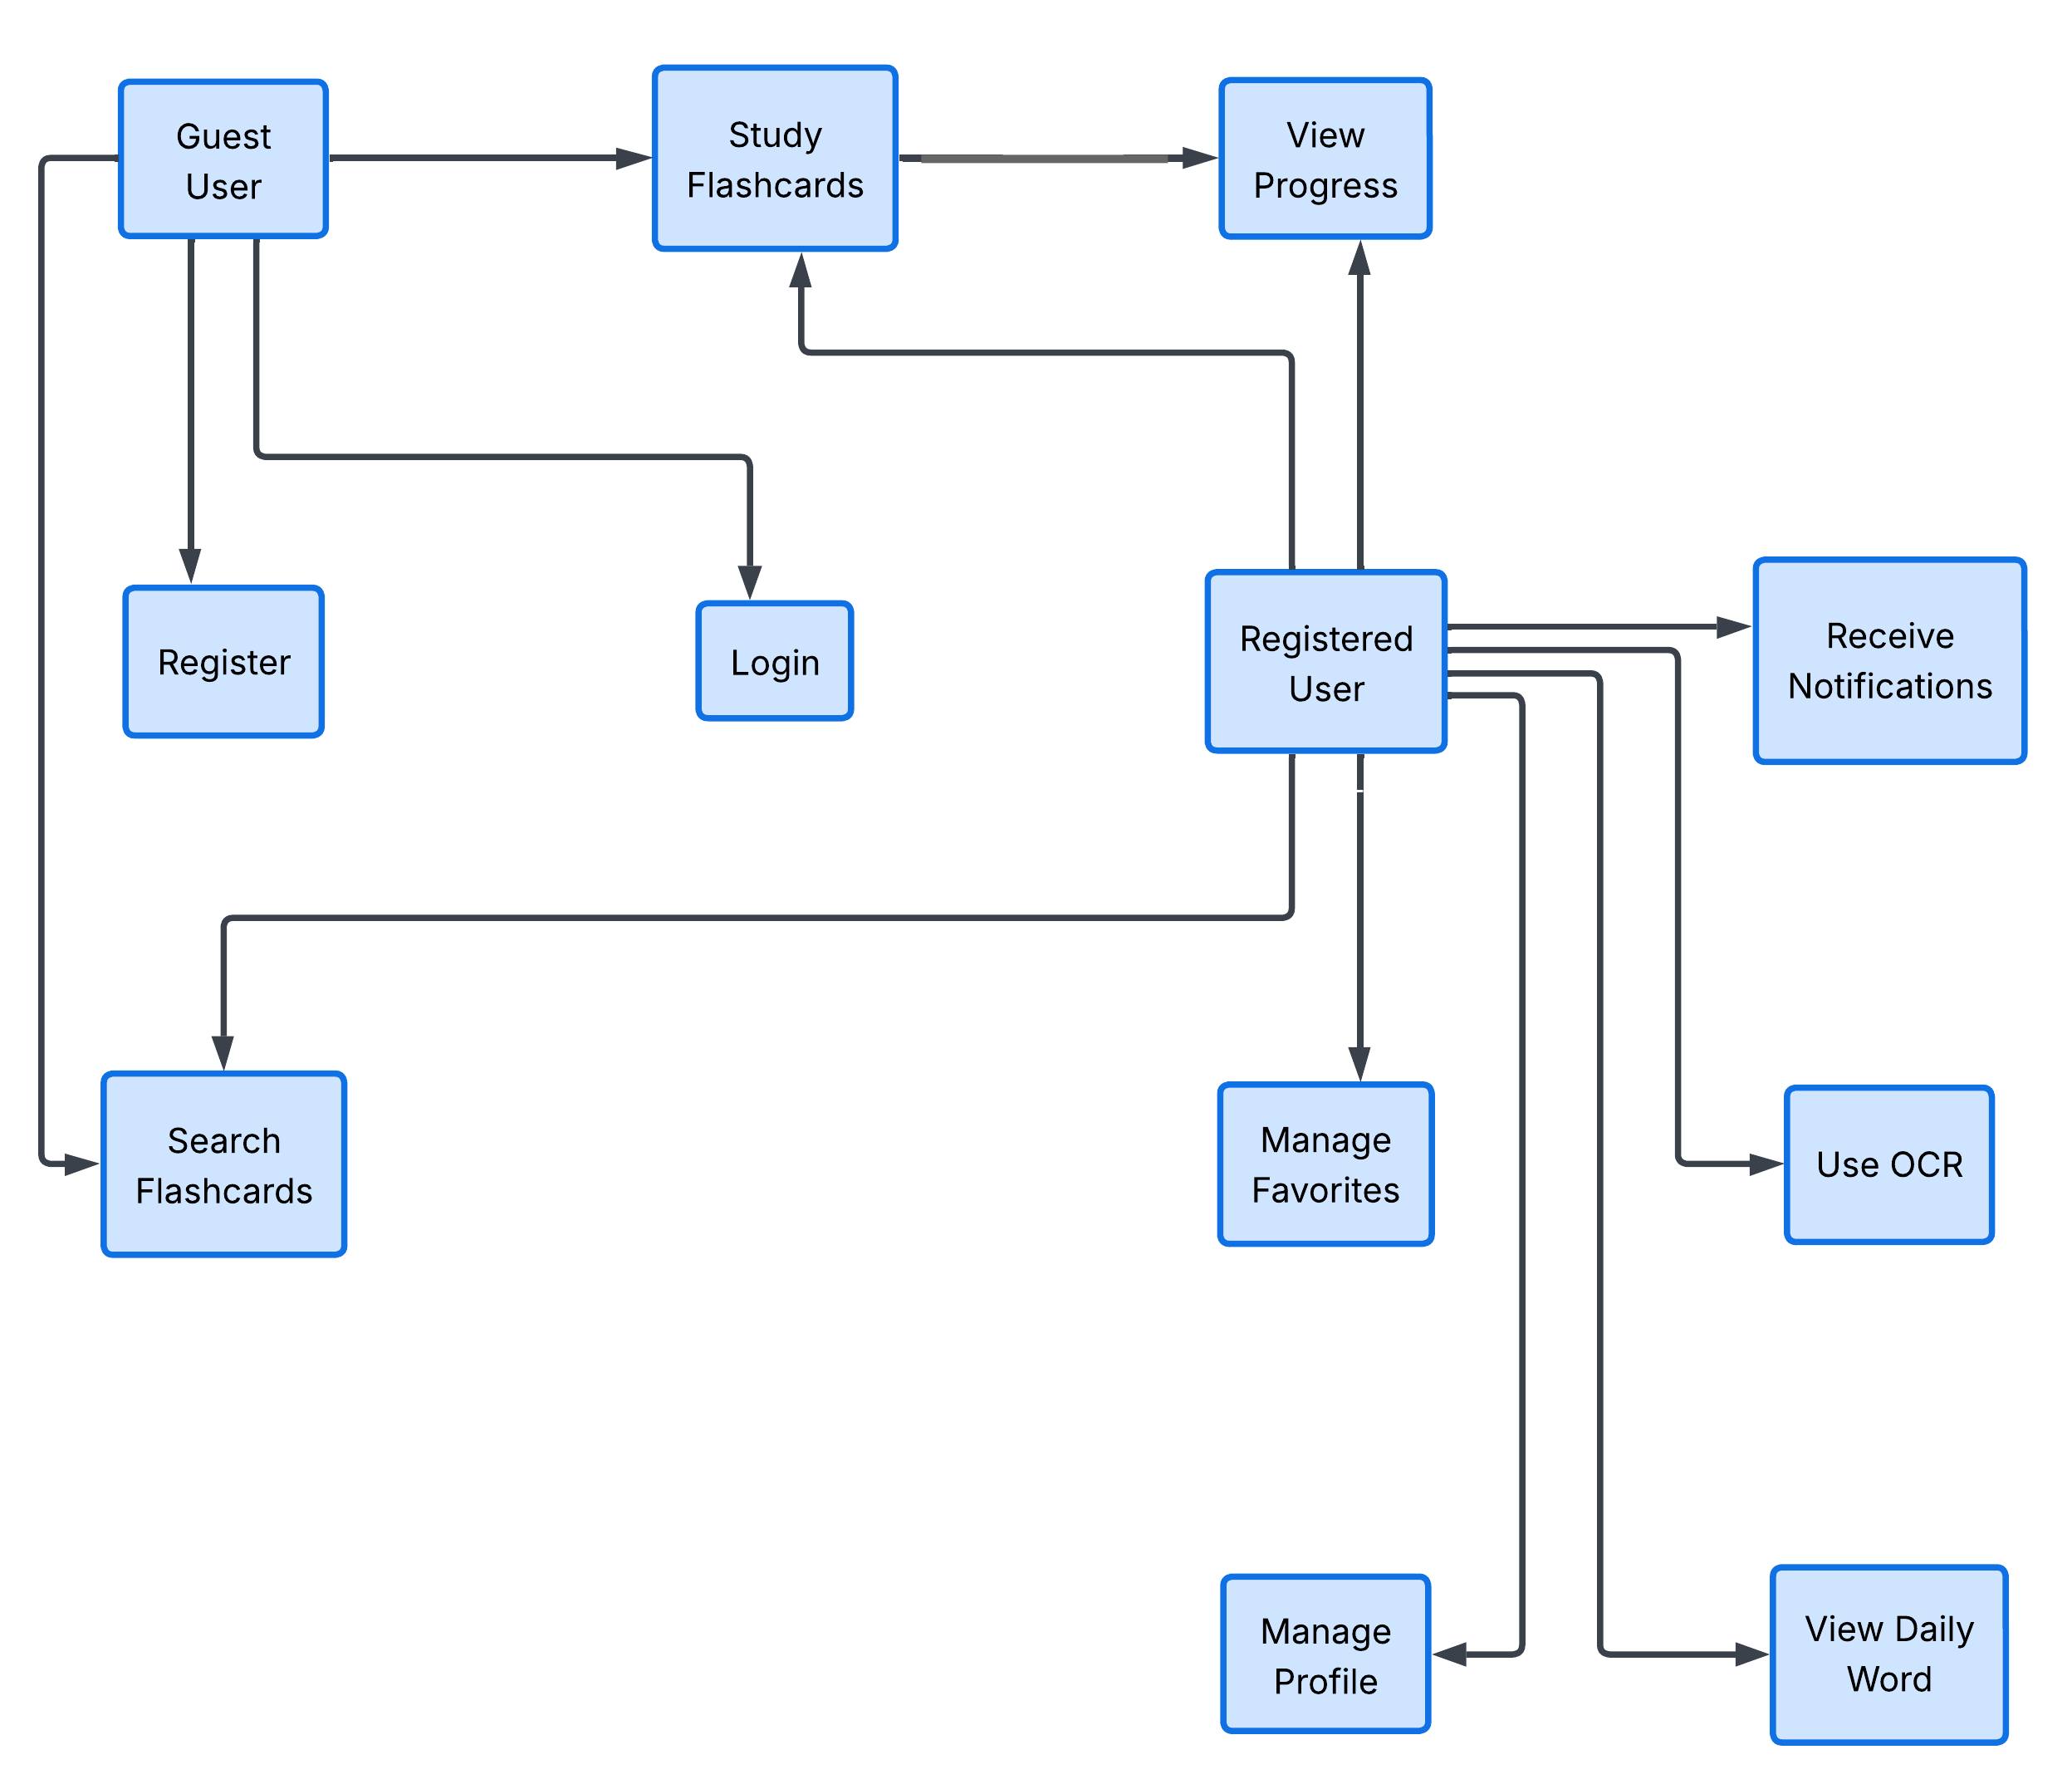
\includegraphics[width=0.68\columnwidth]{Figures/diagrams/usecasediagram.png}
\footnotesize
\captionof{figure}{Системийн use case диаграм}
\label{fig:appendixB-usecase}
\end{center}

Мөн өгөгдлийн урсгалын диаграм нь хэрэглэгчийн оролт, системийн боловсруулалт, өгөгдөл хадгалалт, үр дүн буцаан харуулах үйл явцын хамаарлыг илэрхийлдэг. Жишээлбэл, хэрэглэгч флашкарт дээр хариу өгөхөд тухайн мэдээлэл Firestore-д шинэчлэгдэж, дараагийн давталтын логикт ашиглагдана. OCR-ийн үед хэрэглэгчийн бичсэн дүрсийг боловсруулж, загварт оруулан ангиллын үр дүн буцаадаг.

\begin{center}
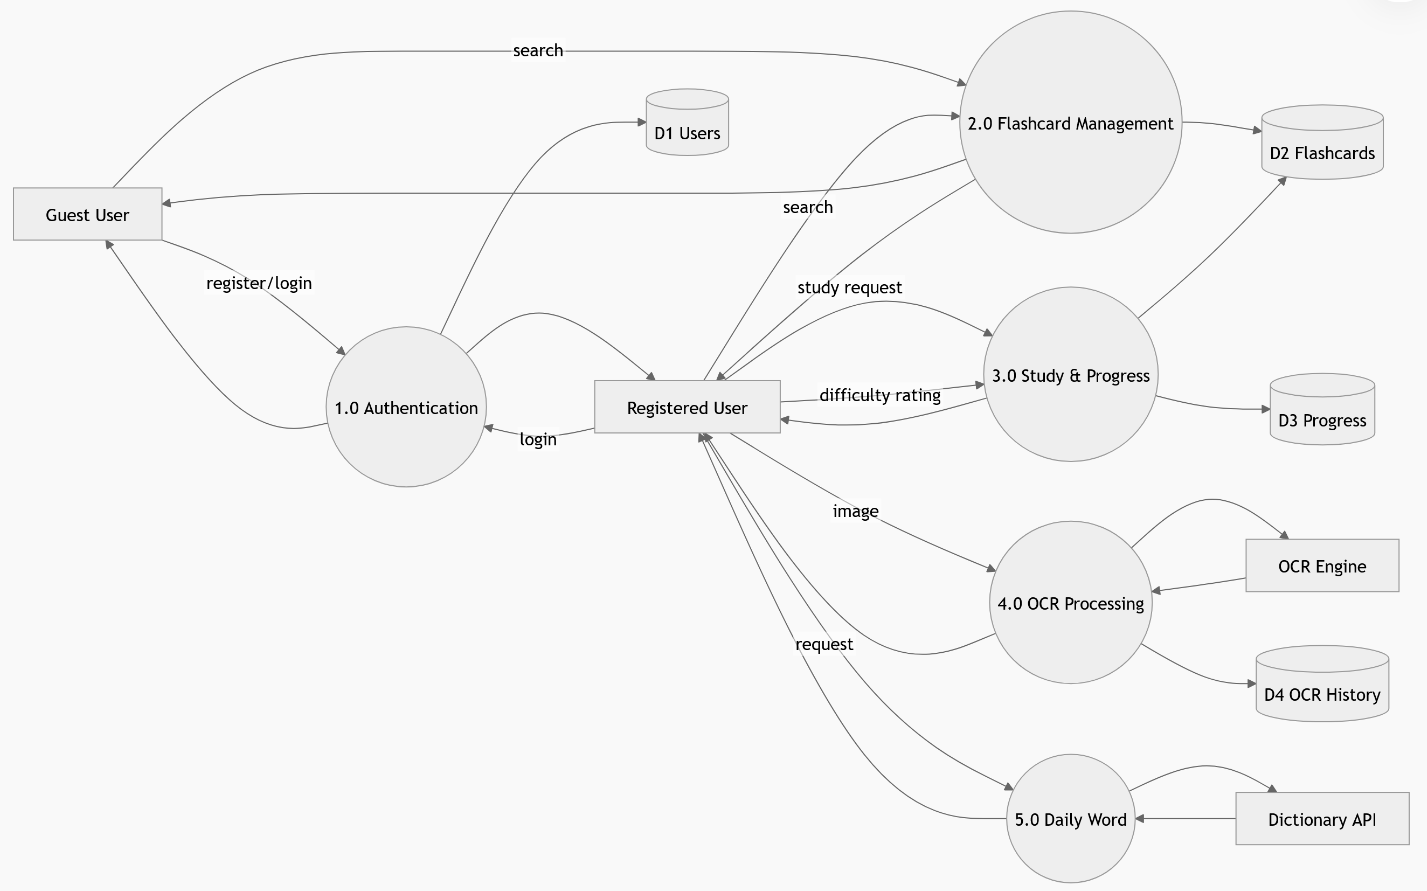
\includegraphics[width=0.68\columnwidth]{Figures/diagrams/dataflow.png}
\footnotesize
\captionof{figure}{Системийн өгөгдлийн урсгалын диаграм}
\label{fig:appendixB-dataflow}
\end{center}
\vspace{-6pt}
OCR системийг хэрэгжүүлэхдээ TensorFlow.js ашигласан. Энэ нь гар бичвэрийн дүрсийг JavaScript орчинд боловсруулж, загвар ашиглан ангилах боломж олгосон. Оролтын зураг нь 28$\times$28 хэмжээтэйгээр боловсруулагдаж, саарал өнгийн хэлбэрт хөрвүүлэгдэн ангилалд оруулсан. Ийнхүү сургалтын орчин болон хиймэл оюунд суурилсан функцийг нэг системд нэгтгэснээр хэрэглэгч зөвхөн хараад сурахаас гадна өөрөө бичиж, шууд шалгах боломжтой болсон.

Судалгааны арга зүйн хувьд системийн шинжилгээ, загварчлал, хэрэгжилт, туршилт гэсэн үе шаттайгаар ажлыг зохион байгуулсан. Эхлээд хэрэглэгчийн хэрэгцээг тодорхойлж, дараа нь use case, data flow, ERD зэрэг диаграмыг боловсруулсан. Үүний дараа интерфейс, өгөгдлийн бүтэц, OCR логикийг үе шаттай хөгжүүлж, эцэст нь гүйцэтгэлийн үр дүнг туршилтын өгөгдлөөр үнэлсэн.

\begin{center}
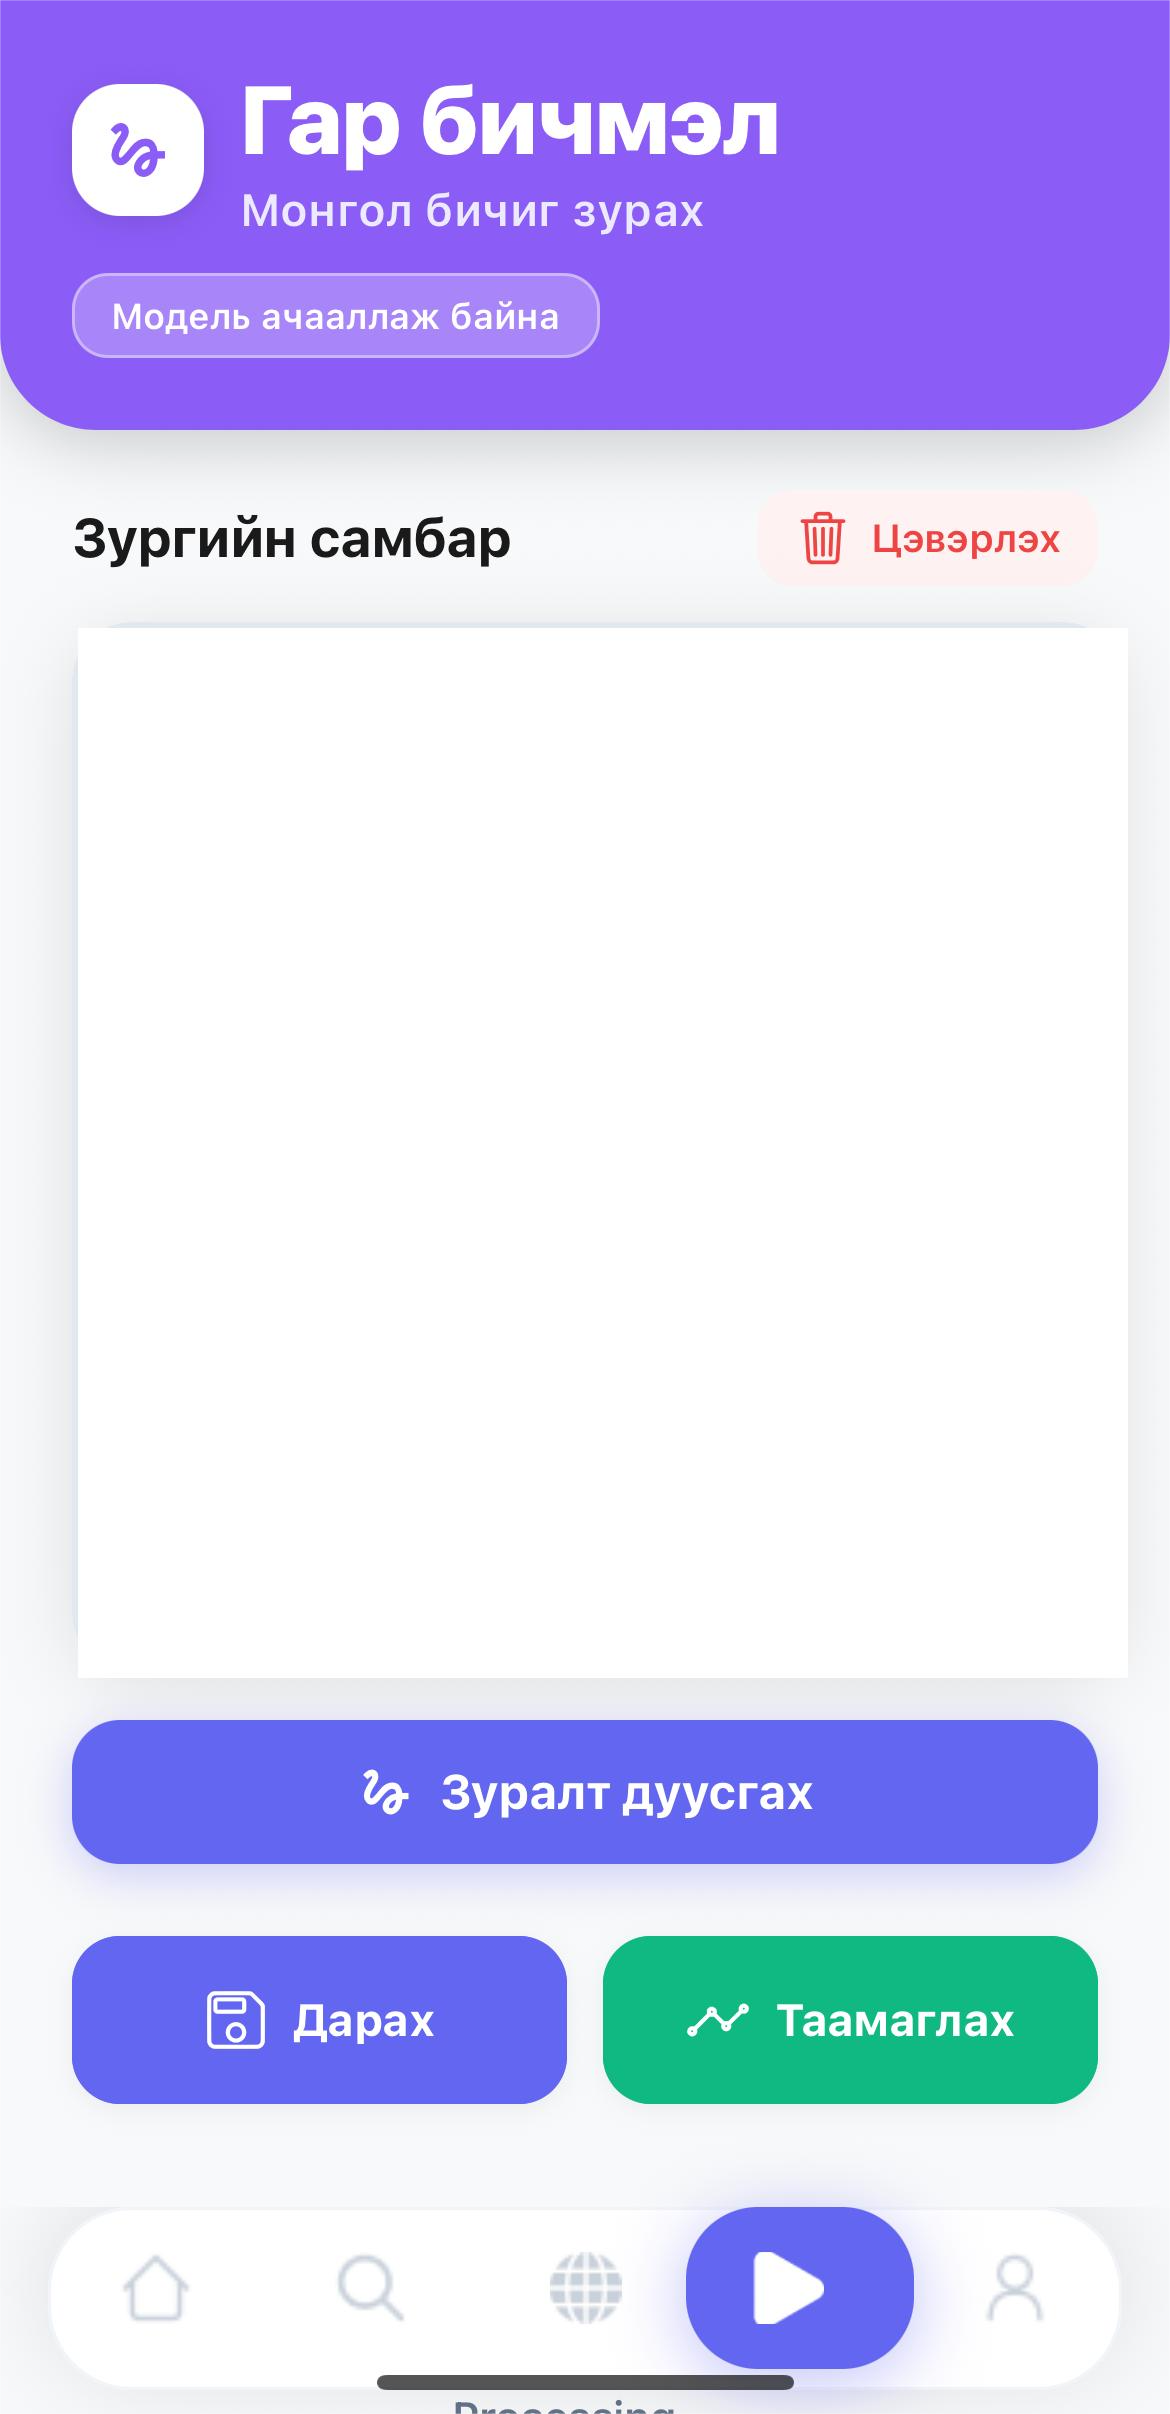
\includegraphics[width=0.62\columnwidth]{Figures/pages/handwriting.png}
\footnotesize
\captionof{figure}{Гараар бичих оролтын дэлгэц}
\label{fig:appendixB-handwriting}
\end{center}

\vspace{-6pt}
\section*{Судалгааны үр дүн}
Системийг хэрэгжүүлсний дараа үндсэн шаардлагуудыг хангаж байгаа эсэхийг хэд хэдэн шалгуураар үнэлсэн. Үүний дүнд апп нь төлөвлөсөн функцуудын дийлэнхийг амжилттай хэрэгжүүлсэн нь тогтоогдсон. Хэрэгжилтийн үндсэн үр дүнг дараах хүснэгтэд харуулав.

\begin{center}
\captionof{table}{Системийн хэрэгжилтийн үр дүн}
\label{tab:appendixB-system-results}
\small
\resizebox{\columnwidth}{!}{%
\begin{tabular}{|l|l|l|}
\hline
\textbf{Шалгуур} & \textbf{Зорилт} & \textbf{Үр дүн} \\
\hline
Платформ & iOS + Android & Амжилттай хэрэгжсэн \\
\hline
Флашкартын тоо & 500+ & 520 \\
\hline
Ангилал & 5+ & 7 ангилал \\
\hline
Хэлний дэмжлэг & 2 хэл & Монгол, Англи \\
\hline
Харагдах горим & Dark/Light & Амжилттай хэрэгжсэн \\
\hline
OCR таних & Монгол бичиг & Үндсэн үсгүүдийг танина \\
\hline
Офлайн горим & Дэмжих & Firestore ашигласан \\
\hline
\end{tabular}}
\end{center}

Хүснэгтээс харахад анхны зорилтуудын хүрээнд тодорхойлсон үндсэн үзүүлэлтүүд бодитоор хэрэгжсэн байна. Ялангуяа флашкартын тоо, ангиллын төрөл, хэлний дэмжлэг, офлайн ажиллагаа зэрэг нь хэрэглэгчийн өдөр тутмын суралцах туршлагыг сайжруулах чухал хүчин зүйл болсон.

OCR загварын гүйцэтгэлийг сургалтын, баталгаажуулалтын болон туршилтын өгөгдлөөр үнэлэхэд дараах үр дүн гарсан.

\begin{itemize}
    \item Training accuracy: 92\%
    \item Validation accuracy: 87\%
    \item Test accuracy: 85\%
    \item Character Error Rate (CER): 15\%
    \item Word Error Rate (WER): 28\%
\end{itemize}

Эдгээр үзүүлэлтээс харахад загвар нь сургалтын өгөгдөл дээр өндөр нарийвчлалтай ажилласан бөгөөд баталгаажуулалтын болон туршилтын өгөгдөл дээрх үр дүн нь хоорондоо хэт зөрүүгүй байна. Энэ нь загварын тогтвортой байдал боломжийн түвшинд байгааг илтгэнэ. Гэсэн хэдий ч WER харьцангуй өндөр байгаа нь үсэг тус бүрийг зөв таньсан ч бүтэн үг түвшинд алдаа гарах магадлал байгааг харуулж байна. Ийм алдаа нь ижил төстэй дүрстэй үсгүүд, өгөгдлийн олон янз байдал хангалтгүй байх, эсвэл гар бичвэрийн ялгаанаас шалтгаалж болно.

\begin{center}
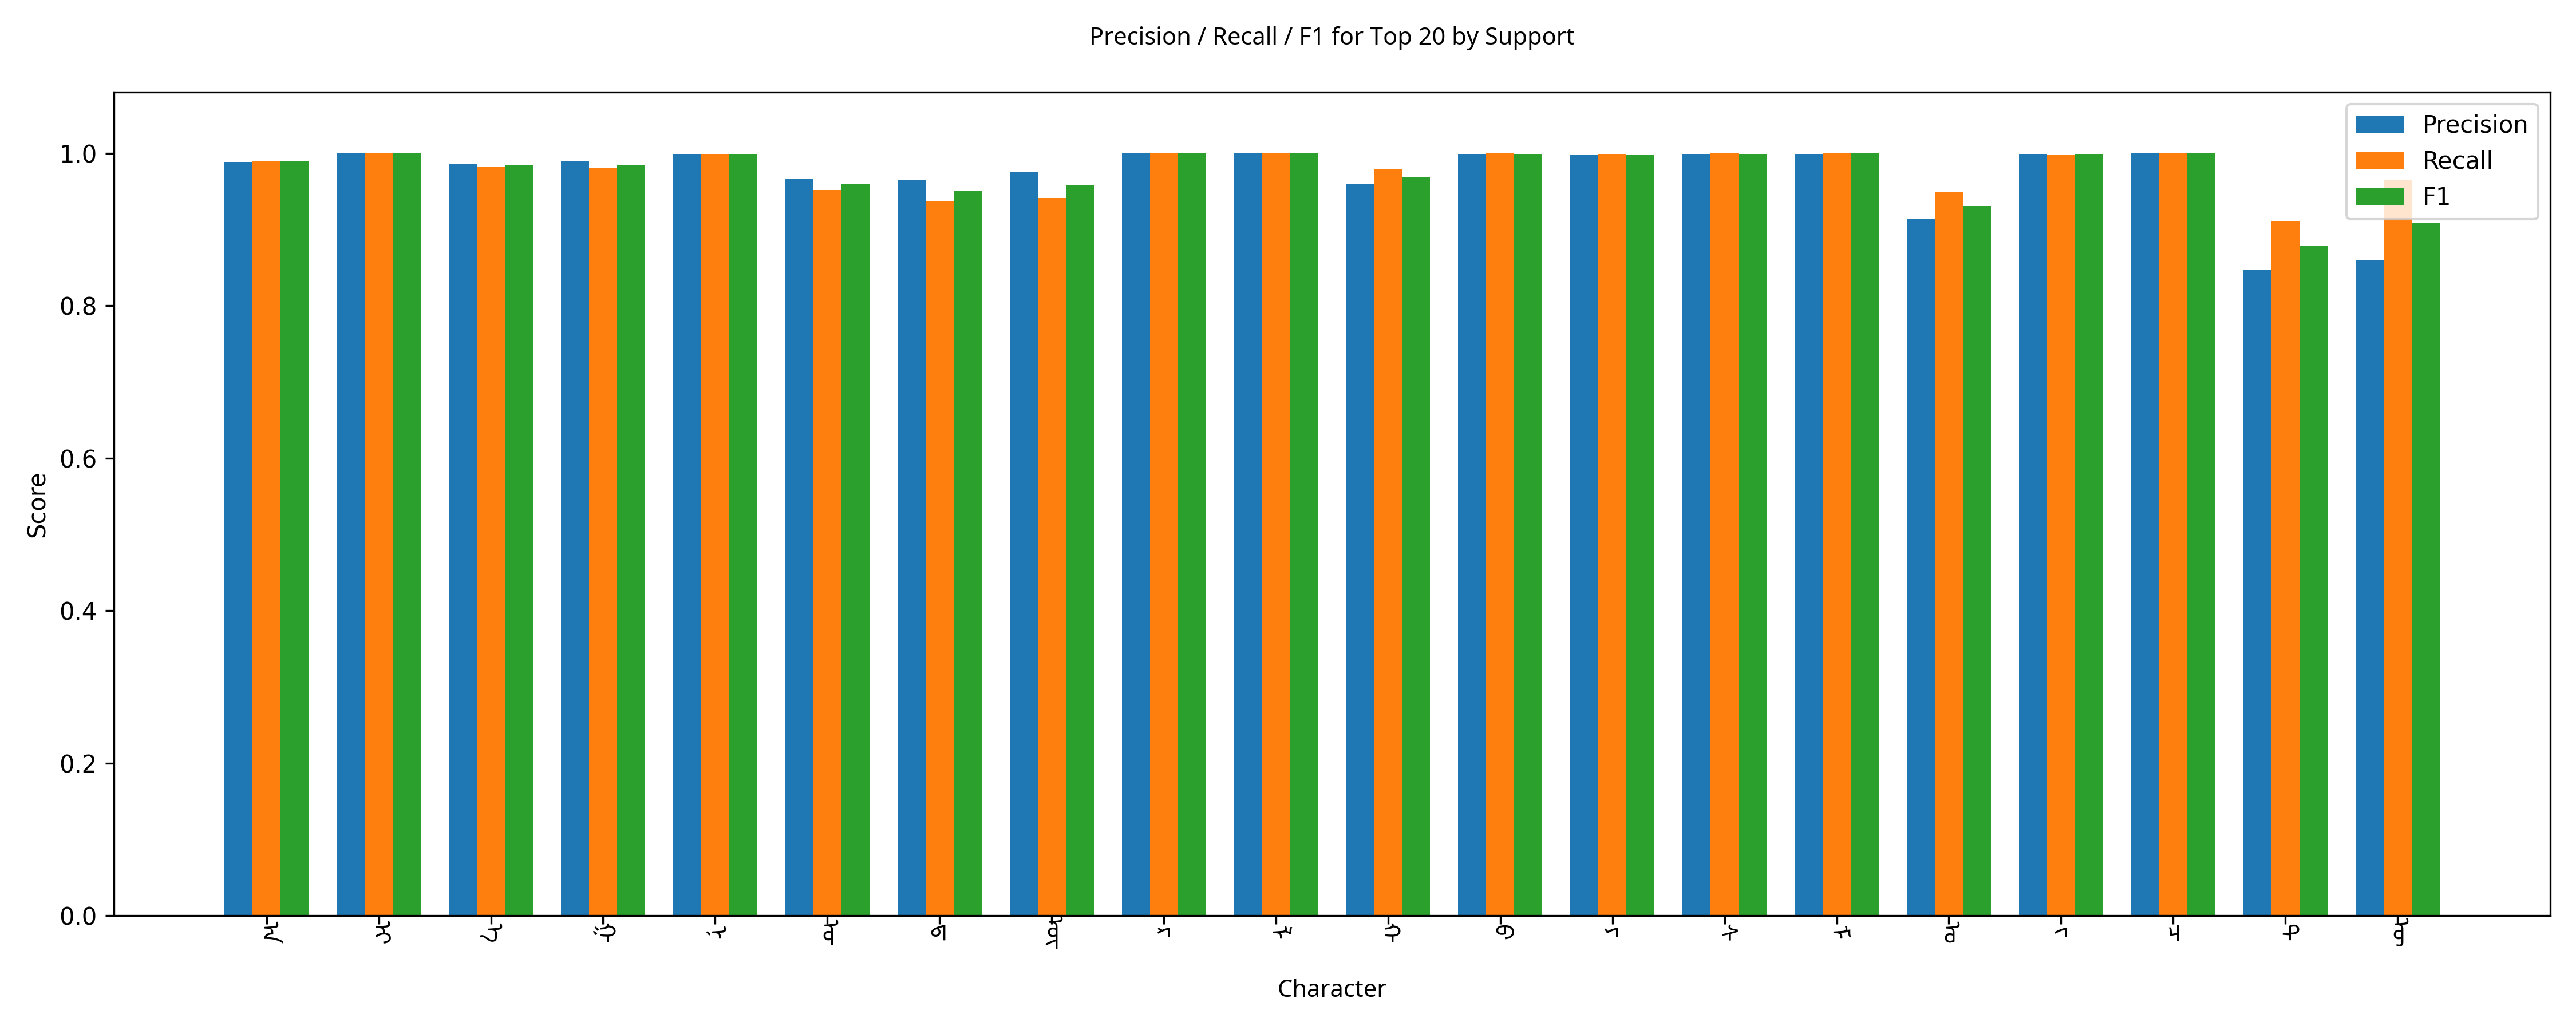
\includegraphics[width=0.66\columnwidth]{Figures/evalution/prf_top_support_clean.png}
\footnotesize
\captionof{figure}{OCR загварын precision, recall, F1 үзүүлэлт}
\label{fig:appendixB-prf}
\end{center}

Загварыг сургахад ашигласан өгөгдлийн бүтэц дараах байдалтай байв.

\begin{center}
\captionof{table}{OCR өгөгдлийн бүтэц}
\label{tab:appendixB-ocr-dataset}
\small
\begin{tabular}{|l|r|}
\hline
\textbf{Өгөгдлийн хэсэг} & \textbf{Тоо} \\
\hline
Сургалтын өгөгдөл & 40000 \\
\hline
Баталгаажуулалтын өгөгдөл & 9615 \\
\hline
Туршилтын өгөгдөл & 20000 \\
\hline
Нийт & 69615 \\
\hline
\end{tabular}
\end{center}

Дээрх өгөгдлийн хэмжээнээс үзэхэд OCR загварыг сургах суурь мэдээлэл хангалттай бүрдсэн боловч бодит хэрэглээний нөхцөлтэй ойртуулахын тулд цаашид гар бичвэрийн төрөл, хэлбэр, зузаан, өнцөг зэрэг олон янзын жишээг нэмэх шаардлагатай. Ингэснээр загварын ерөнхийшүүлэх чадвар сайжирч, бодит хэрэглээний алдаа буурах боломжтой.

Мөн хэрэглэгчийн түвшинд авч үзвэл Egüü апп нь өдөр бүр бага багаар суралцах боломжийг бүрдүүлсэн. Флашкартын давталтын логик, streak, өдрийн үг, ахицын харагдац зэрэг нь хэрэглэгчийг дахин апп руу орж ирэх сэдлийг нэмэгдүүлдэг. Энэ нь зөвхөн технологийн хэрэгжилт бус, боловсролын зориулалттай системийн хувьд хэрэглэгчийн оролцоог нэмэгдүүлэх чухал үр дүн юм.

\vspace{-10pt}
\section*{Судалгааны дүгнэлт}
Энэхүү судалгааны ажлын хүрээнд Egüü нэртэй монгол бичгийн сургалтын аппликейшнийг амжилттай боловсруулж, үндсэн функцуудыг хэрэгжүүллээ. Систем нь кросс-платформ орчинд ажиллах боломжтой, хэрэглэгчийн өгөгдлийг найдвартай хадгалах бүтэцтэй, мөн OCR-д суурилсан гар бичвэр таних чадвартай болсон нь энэхүү ажлын гол үр дүн юм.

Флашкартын систем, OCR технологи, хэрэглэгчийн статистик, хоёр хэлний дэмжлэг зэрэг функцийг нэг дор уялдуулснаар монгол бичиг сурах үйл явцыг илүү уян хатан, сонирхолтой, үр өгөөжтэй болгож чадсан. Түүнчлэн Firebase орчин ашигласнаар өгөгдлийн төвлөрсөн удирдлага, хэрэглэгч хоорондын ялгаатай ахицыг хадгалах боломж бүрдсэн.

Судалгааны үр дүнгээс харахад систем нь боловсролын технологийн практик хэрэглээний жишээ болох боломжтой бөгөөд цаашид илүү өргөн хэрэглээнд нэвтрүүлэх суурьтай байна. Ялангуяа OCR-ийн нарийвчлалыг сайжруулах, флашкартын дасан зохицох алгоритмыг нэмэгдүүлэх, шагналт механизмыг оруулах, хамтран суралцах боломж нэмэх зэрэг нь ирээдүйн хөгжүүлэлтийн чухал чиглэл болно.

Иймээс Egüü апп нь монгол бичгийг хадгалан түгээн дэлгэрүүлэх үйл хэрэгт хувь нэмэр оруулахын зэрэгцээ, мэдээллийн технологийг эх хэл, өв соёлын боловсролд ашиглах бодит шийдэл болж чадна гэж дүгнэж байна.

\vspace{-12pt}
\enlargethispage{2\baselineskip}
\section*{Ном зүй}
\vspace{-6pt}
{\scriptsize
\printbibliography[heading=none]
}
\end{multicols}

